\chapter{APPENDICES}

\renewcommand{\headrulewidth}{0.5pt}
\renewcommand{\footrulewidth}{0.5pt}
\thispagestyle{plain}
\pagestyle{fancy}
\fancyhf{}
\fancyhead[L]{\textbf{CHAPTER 6}}
\fancyhead[R]{\textbf{DROWSINESS DETECTION AND ALERT SYSTEM IN THE CAR}}
\raggedright
\fancyfoot[L]{From: Nguyen Van Anh Tuan}
\fancyfoot[R]{Page \thepage}

\justifying

\definecolor{mygray}{rgb}{0.5,0.5,0.5}

\section{Drowsiness Detection Program}

    \lstset{ 
        backgroundcolor=\color{white},   % choose the background color; you must add \usepackage{color} or \usepackage{xcolor}; should come as last argument
        basicstyle=\footnotesize,        % the size of the fonts that are used for the code
        breakatwhitespace=false,         % sets if automatic breaks should only happen at whitespace
        breaklines=true,                 % sets automatic line breakingcommentstyle=\color{mygreen},    % comment style
        captionpos=b,
        deletekeywords={...},            % if you want to delete keywords from the given language
        escapeinside={\%*}{*)},          % if you want to add LaTeX within your code
        extendedchars=true,              % lets you use non-ASCII characters; for 8-bits encodings only, does not work with UTF-8
        firstnumber=1,                % start line enumeration with line 1
        frame=single,	                   % adds a frame around the code
        keepspaces=true,                 % keeps spaces in text, useful for keeping indentation of code (possibly needs columns=flexible)
        keywordstyle=\color{blue},       % keyword style
        language=Python,                 % the language of the code
        morekeywords={*,...},            % if you want to add more keywords to the set
        numbers=left,                    % where to put the line-numbers; possible values are (none, left, right)
        numbersep=5pt,                   % how far the line-numbers are from the code
        numberstyle=\tiny\color{mygray}, % the style that is used for the line-numbers
        rulecolor=\color{black},         % if not set, the frame-color may be changed on line-breaks within not-black text (e.g. comments (green here))
        showspaces=false,                % show spaces everywhere adding particular underscores; it overrides 'showstringspaces'
        showstringspaces=false,          % underline spaces within strings only
        showtabs=false,                  % show tabs within strings adding particular underscores
        stepnumber=1,                    % the step between two line-numbers. If it's 1, each line will be numberedstringstyle=\color{mymauve},     % string literal style
        tabsize=2,	                   % sets default tabsize to 2 spaces
        title=\lstname                   % show the filename of files included with \lstinputlisting; also try caption instead of title
    }

    \begin{lstlisting}[caption={Import library}]
        from imutils.video import VideoStream
        from imutils import face_utils
        import numpy as np
        import argparse
        import imutils
        import playsound
        import time
        from threading import Thread
        import dlib
        import os
        import cv2
    \end{lstlisting}

    \begin{lstlisting}[caption={Setup sound file and turn it on}]
        wav_path = "/Drowsiness/alarm.wav"
        def play_sound(path):
            os.system('play' + path)
    \end{lstlisting}

    \begin{lstlisting}[caption={Compute the distance between 2 point A and B}]
        def e_dist(pA, pB):
            return np.linalg.norm(pA - pB)
        def eye_ratio(eye):
            #Khoang cach theo chieu doc mi tren va mi duoi
            d_V1 = e_dist(eye[1], eye[5])
            d_V2 = e_dist(eye[2], eye[4])
        
            #Khoang cach theo chieu ngang giua 2 mat
            d_H = e_dist(eye[0], eye[3])
        
            #Ty le giua chieu doc va ngang
            eye_ratio_val = (d_V1 + d_V2) / (2.0 * d_H)
            
            return eye_ratio_val
    \end{lstlisting}

    \begin{lstlisting}[caption={Define threshold level. If smaller than this is drowsiness}]
        eye_ratio_threshold = 0.25
    \end{lstlisting}

    \begin{lstlisting}[caption={Threshold so frame lien tuc nham mat}]
        max_sleep_frames = 16
    \end{lstlisting}

    \begin{lstlisting}[caption={Dem so frame ngu}]
        sleep_frames = 0
    \end{lstlisting}

    \begin{lstlisting}[caption={Check xem da canh bao hay chua}]
        alarmed = False 
    \end{lstlisting}

    \begin{lstlisting}[caption={Khoi tao cac module detect mat va facial landmark}]
        face_detect = cv2.CascadeClassifier("haarcascade_frontalface_default.xml")
        landmark_detect = dlib.shape_predictor("shape_predictor_68_face_landmarks.dat")
    \end{lstlisting}

    \begin{lstlisting}[caption={Lay danh sach cac cum diem landmark cho 2 mat}]
        (left_eye_start, left_eye_end) = face_utils.FACIAL_LANDMARKS_IDXS["left_eye"]
        (right_eye_start, right_eye_end) = face_utils.FACIAL_LANDMARKS_IDXS["right_eye"]
    \end{lstlisting}

    \begin{lstlisting}[caption={Doc tu camera}]
        vs = VideoStream(src=0).start()
        time.sleep(1.0)

        while True:

            # Doc tu camera
            frame = vs.read()

            # Resize de tang toc do xu ly
            frame = imutils.resize(frame, width=450)

            # Chuyen ve gray
            gray = cv2.cvtColor(frame, cv2.COLOR_BGR2GRAY)

            # Detect cac mat trong anh
            faces = face_detect.detectMultiScale(gray, scaleFactor=1.1,	minNeighbors=5, minSize=(100, 100),	flags=cv2.CASCADE_SCALE_IMAGE)

            # Duyet qua cac mat
            for (x, y, w, h) in faces:

                # Tao mot hinh chu nhat quanh khuon mat
                rect = dlib.rectangle(int(x), int(y), int(x + w),
                    int(y + h))

                # Nhan dien cac diem landmark
                landmark = landmark_detect(gray, rect)
                landmark = face_utils.shape_to_np(landmark)

                # Tinh toan ty le mat phai va trai va trung binh cong 2 ratio
                leftEye = landmark[left_eye_start:left_eye_end]
                rightEye = landmark[right_eye_start:right_eye_end]

                left_eye_ratio = eye_ratio(leftEye)
                right_eye_ratio = eye_ratio(rightEye)

                eye_avg_ratio = (left_eye_ratio + right_eye_ratio) / 2.0

                # Ve duong bao quanh mat
                left_eye_bound = cv2.convexHull(leftEye)
                right_eye_bound = cv2.convexHull(rightEye)
                cv2.drawContours(frame, [left_eye_bound], -1, (0, 255, 0), 1)
                cv2.drawContours(frame, [right_eye_bound], -1, (0, 255, 0), 1)

                # Check xem mat co nham khong
                if eye_avg_ratio < eye_ratio_threshold:
                    sleep_frames += 1
                    # if the eyes were closed for a sufficient number of
                    # frames, then sound the alarm
                    if sleep_frames >= max_sleep_frames:

                        if not alarmed:
                            alarmed = True
                            # Duong dan den file wav


                            # Tien hanh phat am thanh trong 1 luong rieng
                            t = Thread(target=play_sound,
                                        args=(wav_path,))
                            t.deamon = True
                            t.start()

                        # Ve dong chu canh bao
                        cv2.putText(frame, "DROWSINESS ALERT", (10, 30), cv2.FONT_HERSHEY_SIMPLEX, 0.7, (0, 0, 255), 2)

                # Neu khong nham mat thi
                else:

                    # Reset lai cac tham so
                    sleep_frames = 0
                    alarmed = False

                    # Hien thi gia tri eye ratio trung binh
                    cv2.putText(frame, "EYE AVG RATIO: {:.3f}".format(eye_avg_ratio), (10, 30),	cv2.FONT_HERSHEY_SIMPLEX, 0.7, (255, 0, 0), 2)

            # Hien thi len man hinh
            cv2.imshow("Camera", frame)

            # Bam Esc de thoat
            key = cv2.waitKey(1) & 0xFF
            if key == 27:
                break
    \end{lstlisting}

    \begin{lstlisting}[caption={End program}]
        cv2.destroyAllWindows()
        vs.stop()
    \end{lstlisting}

\section{Install Raspbian OS for Raspberry Pi 3B+}
    Require equipment for installation: 
    \begin{itemize}
        \item Micro SDHC card 32GB + adapter 
        \item Laptop for installation 
        \item Monitor 
        \item LAN cable for convenient remote control by laptop
        \item Power 5v, 2.5A (at least 1A) 
    \end{itemize}
    \subsection{Step 1}
        Download Raspbian OS ISO file to laptop and extract it
        \begin{figure}[H]
            \centering
            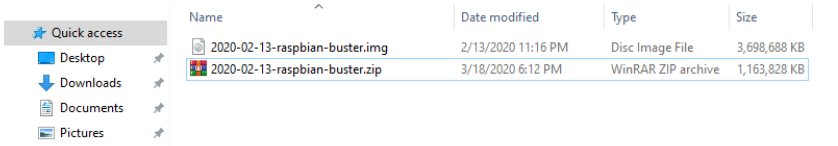
\includegraphics[width=0.6\linewidth]{img/download.PNG}
            \caption{The file contain Raspbian OS}
        \end{figure}
    \subsection{Step 2}
        Install SD card formater and win32 Disk Imager software
    \subsection{Step 3}
        Insert MicroSD card into card reader in laptop and check drive name of disk assigned to memory card to avoid 
        confusion causing other data loss. 
    \subsection{Step 4}
        Run SD Card Formater software to format memory card then run Win32 Disk Imager start install OS to the memory card
        \begin{figure}[H]
            \centering
            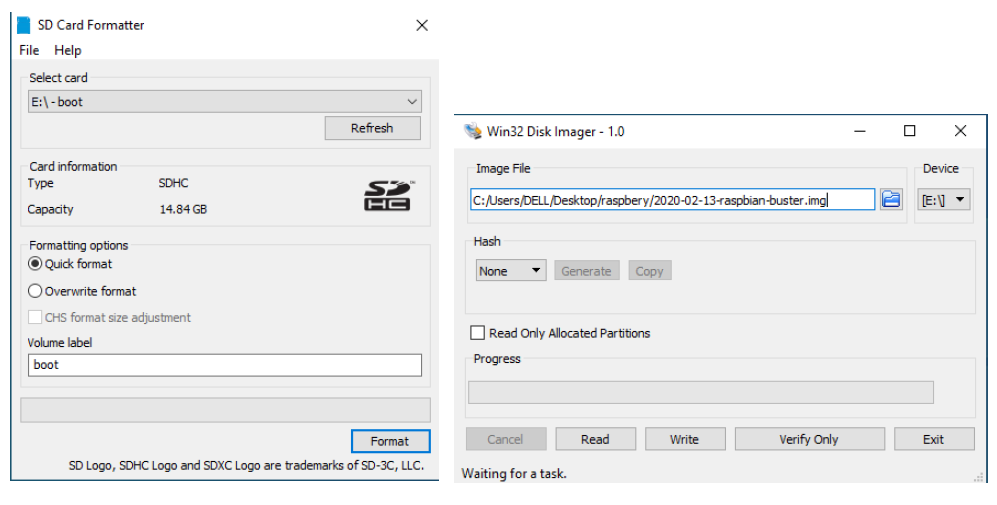
\includegraphics[width=0.6\linewidth]{img/format-disk.PNG}
            \caption{Format disk and install OS into memory card}
        \end{figure}
\section{Install Necessary Libraries}
    \subsection{OpenCV}
        \textbf{\$sudo apt install python3-pip} \\ 
        \vspace{3mm}
        This step allow us to install pip in Python 3. Next we using Pip command to install OpenCV library by using: \\ 
        \vspace{3mm}
        \textbf{\$sudo pip3 install opencv-python} \\ 
        \vspace{3mm}
        Next we install another package to run the code: 
        \begin{itemize}
            \item imutils
            \item numpy
            \item playsound 
            \item dlib
        \end{itemize}
\section{Run program}
    At last, we run this command to run program with 2 components is sound file and data file of HaarCascade front face: \\
    \vspace{3mm}
    \textbf{\$python3 main.py}
    \begin{figure}[H]
        \centering
        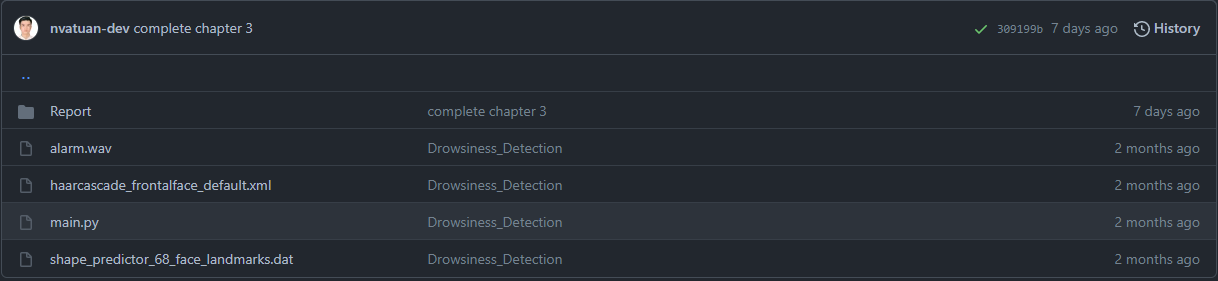
\includegraphics[width=0.8\linewidth]{img/folder-tree.PNG}
        \caption{Folder tree of project}
    \end{figure}